
\documentclass[a4paper,11pt,twoside]{ThesisStyle}

%\usepackage{graphicx}
\usepackage{fancyvrb}
\bibliographystyle{unsrt}
\usepackage{url}
\usepackage{listings}
\usepackage{tabularx}
\usepackage{pdflscape}
\usepackage{subfigure}

%\newcommand{\todo}[1]{\noindent\textcolor{red}{{\bf \{TODO}: #1{\bf \}}}}
\newcommand{\ghis}[1]{\noindent\textcolor{blue}{{\bf \{Ghis}: #1{\bf \}}}}

\usepackage{amsmath,amssymb}             % AMS Math
% \usepackage[french]{babel}
\usepackage[latin1]{inputenc}
\usepackage[T1]{fontenc}
\usepackage[left=1.5in,right=1.3in,top=1.1in,bottom=1.1in,includefoot,includehead,headheight=13.6pt]{geometry}
\renewcommand{\baselinestretch}{1.05}

% Table of contents for each chapter

\usepackage[nottoc, notlof, notlot]{tocbibind}
\usepackage{minitoc}
\setcounter{minitocdepth}{2}
\mtcindent=15pt
% Use \minitoc where tos put a table of contents

\usepackage{aecompl}

% Glossary / list of abbreviations

\usepackage[intoc]{nomencl}
\renewcommand{\nomname}{List of Abbreviations}

\makenomenclature

% My pdf code

\usepackage{ifpdf}

\ifpdf
  \usepackage[pdftex]{graphicx}
  \DeclareGraphicsExtensions{.jpg}
  \usepackage[a4paper,pagebackref,hyperindex=true]{hyperref}
\else
  \usepackage{graphicx}
  \DeclareGraphicsExtensions{.ps,.eps}
  \usepackage[a4paper,dvipdfm,pagebackref,hyperindex=true]{hyperref}
\fi

\graphicspath{{.}{images/}}

% Links in pdf
\usepackage{color}
\definecolor{linkcol}{rgb}{0,0,0.4} 
\definecolor{citecol}{rgb}{0.5,0,0} 

% Change this to change the informations included in the pdf file

% See hyperref documentation for information on those parameters

\hypersetup
{
bookmarksopen=true,
pdftitle="First class futures",
pdfauthor="Muhammad Uzair KHAN", 
pdfsubject="update strategies for first class futures", %subject of the document
%pdftoolbar=false, % toolbar hidden
pdfmenubar=true, %menubar shown
pdfhighlight=/O, %effect of clicking on a link
colorlinks=true, %couleurs sur les liens hypertextes
pdfpagemode=None, %aucun mode de page
pdfpagelayout=SinglePage, %ouverture en simple page
pdffitwindow=true, %pages ouvertes entierement dans toute la fenetre
linkcolor=linkcol, %couleur des liens hypertextes internes
citecolor=citecol, %couleur des liens pour les citations
urlcolor=linkcol %couleur des liens pour les url
}

% definitions.
% -------------------

\setcounter{secnumdepth}{3}
\setcounter{tocdepth}{2}

% Some useful commands and shortcut for maths:  partial derivative and stuff

\usepackage [table]{xcolor}


\newcommand{\pd}[2]{\frac{\partial #1}{\partial #2}}
\def\abs{\operatorname{abs}}
\def\argmax{\operatornamewithlimits{arg\,max}}
\def\argmin{\operatornamewithlimits{arg\,min}}
\def\diag{\operatorname{Diag}}
\newcommand{\eqRef}[1]{(\ref{#1})}

\usepackage{rotating}                    % Sideways of figures & tables
%\usepackage{bibunits}
%\usepackage[sectionbib]{chapterbib}          % Cross-reference package (Natural BiB)
%\usepackage{natbib}                  % Put References at the end of each chapter
                                         % Do not put 'sectionbib' option here.
                                         % Sectionbib option in 'natbib' will do.
\usepackage{fancyhdr}                    % Fancy Header and Footer

% \usepackage{txfonts}                     % Public Times New Roman text & math font
  
%%% Fancy Header %%%%%%%%%%%%%%%%%%%%%%%%%%%%%%%%%%%%%%%%%%%%%%%%%%%%%%%%%%%%%%%%%%
% Fancy Header Style Options

\pagestyle{fancy}                       % Sets fancy header and footer
\fancyfoot{}                            % Delete current footer settings

%\renewcommand{\chaptermark}[1]{         % Lower Case Chapter marker style
%  \markboth{\chaptername\ \thechapter.\ #1}}{}} %

%\renewcommand{\sectionmark}[1]{         % Lower case Section marker style
%  \markright{\thesection.\ #1}}         %

\fancyhead[LE,RO]{\bfseries\thepage}    % Page number (boldface) in left on even
% pages and right on odd pages
\fancyhead[RE]{\bfseries\nouppercase{\leftmark}}      % Chapter in the right on even pages
\fancyhead[LO]{\bfseries\nouppercase{\rightmark}}     % Section in the left on odd pages

\let\headruleORIG\headrule
\renewcommand{\headrule}{\color{black} \headruleORIG}
\renewcommand{\headrulewidth}{1.0pt}
\usepackage{colortbl}
\arrayrulecolor{black}

\fancypagestyle{plain}{
  \fancyhead{}
  \fancyfoot{}
  \renewcommand{\headrulewidth}{0pt}
}

%\usepackage{algorithm}
%\usepackage{algorithmic}
%\usepackage[ruled,vlined]{algorithm2e}
%%% Clear Header %%%%%%%%%%%%%%%%%%%%%%%%%%%%%%%%%%%%%%%%%%%%%%%%%%%%%%%%%%%%%%%%%%
% Clear Header Style on the Last Empty Odd pages
\makeatletter

\def\cleardoublepage{\clearpage\if@twoside \ifodd\c@page\else%
  \hbox{}%
  \thispagestyle{empty}%              % Empty header styles
  \newpage%
  \if@twocolumn\hbox{}\newpage\fi\fi\fi}

\makeatother
 
%%%%%%%%%%%%%%%%%%%%%%%%%%%%%%%%%%%%%%%%%%%%%%%%%%%%%%%%%%%%%%%%%%%%%%%%%%%%%%% 
% Prints your review date and 'Draft Version' (From Josullvn, CS, CMU)
\newcommand{\reviewtimetoday}[2]{\special{!userdict begin
    /bop-hook{gsave 20 710 translate 45 rotate 0.8 setgray
      /Times-Roman findfont 12 scalefont setfont 0 0   moveto (#1) show
      0 -12 moveto (#2) show grestore}def end}}
% You can turn on or off this option.
% \reviewtimetoday{\today}{Draft Version}
%%%%%%%%%%%%%%%%%%%%%%%%%%%%%%%%%%%%%%%%%%%%%%%%%%%%%%%%%%%%%%%%%%%%%%%%%%%%%%% 

\newenvironment{maxime}[1]
{
\vspace*{0cm}
\hfill
\begin{minipage}{0.5\textwidth}%
%\rule[0.5ex]{\textwidth}{0.1mm}\\%
\hrulefill $\:$ {\bf #1}\\
%\vspace*{-0.25cm}
\it 
}%
{%

\hrulefill
\vspace*{0.5cm}%
\end{minipage}
}

\let\minitocORIG\minitoc
\renewcommand{\minitoc}{\minitocORIG \vspace{1.5em}}

\usepackage{multirow}
%\usepackage{slashbox}

\newenvironment{bulletList}%
{ \begin{list}%
	{$\bullet$}%
	{\setlength{\labelwidth}{25pt}%
	 \setlength{\leftmargin}{30pt}%
	 \setlength{\itemsep}{\parsep}}}%
{ \end{list} }

\newtheorem{definition}{D�finition}
\renewcommand{\epsilon}{\varepsilon}

% centered page environment

\newenvironment{vcenterpage}
{\newpage\vspace*{\fill}\thispagestyle{empty}\renewcommand{\headrulewidth}{0pt}}
{\vspace*{\fill}}
\usepackage{verbatim}
%\usepackage{minitoc}
%\usepackage{wrapfig}
\usepackage{listings}
\usepackage{hyperref}
\hypersetup{
    bookmarks=true,         % show bookmarks bar?
    unicode=false,          % non-Latin characters in Acrobat�s bookmarks
    pdftoolbar=true,        % show Acrobat�s toolbar?
    pdfmenubar=true,        % show Acrobat�s menu?
    pdffitwindow=false,     % window fit to page when opened
    pdfstartview={FitH},    % fits the width of the page to the window
    pdftitle={My title},    % title
    pdfauthor={Author},     % author
    pdfsubject={Subject},   % subject of the document
    pdfcreator={Creator},   % creator of the document
    pdfproducer={Producer}, % producer of the document
    pdfkeywords={keyword1} {key2} {key3}, % list of keywords
    pdfnewwindow=true,      % links in new window
    colorlinks=false,       % false: boxed links; true: colored links
    linkcolor=red,          % color of internal links
    citecolor=green,        % color of links to bibliography
    filecolor=magenta,      % color of file links
    urlcolor=cyan           % color of external links
}

\newcommand{\todo}[1]{\textcolor{red}{%
\raisebox{-0.2em}[0pt][0pt]{\makebox[0pt]{\rule{1pt}{1.1em}}\makebox[0pt][l]{\raisebox{1em}{\rule{5ex}{1pt}}}}
\textbf{TODO:} \textit{#1}
\raisebox{-0.2em}[0pt][0pt]{\makebox[0pt][r]{\rule{5ex}{1pt}}\makebox[0pt]{\rule{1pt}{1em}}}%
}}

\newcommand{\comments}[1]{\textcolor{blue}{%
\raisebox{-0.2em}[0pt][0pt]{\makebox[0pt]{\rule{1pt}{1.1em}}\makebox[0pt][l]{\raisebox{1em}{\rule{5ex}{1pt}}}}
\textbf{COMMENTS:} \textit{#1}
\raisebox{-0.2em}[0pt][0pt]{\makebox[0pt][r]{\rule{5ex}{1pt}}\makebox[0pt]{\rule{1pt}{1em}}}%
}}

%\usepackage[dvips]{graphicx, color}
%\usepackage[bookmarks=true, bookmarksnumbered=true,hypertexnames=false, breaklinks=true]{hyperref}
%\DeclareGraphicsExtensions{.eps,.ps}

\newlength{\plarg}
\setlength{\plarg}{16cm}
\newlength{\glarg}
\setlength{\glarg}{17cm}
\lstset{
         basicstyle=\scriptsize\ttfamily, % Standardschrift
         numbers=left,               % Ort der Zeilennummern
         numberstyle=\tiny,          % Stil der Zeilennummern
         frame=single,
         %stepnumber=2,               % Abstand zwischen den Zeilennummern
         numbersep=5pt,              % Abstand der Nummern zum Text
         tabsize=2,                  % Groesse von Tabs
         extendedchars=true,         %
         breaklines=true,            % Zeilen werden Umgebrochen
         keywordstyle=\color{red},
                frame=b,         
  %       keywordstyle=[1]\textbf,    ]{\index{keywords, BEGIN}}% Stil der Keywords
  %       keywordstyle=[2]\textbf,    %
  %      keywordstyle=[3]\textbf,    %
 %        keywordstyle=[4]\textbf,   \sqrt{\sqrt{}} %
         stringstyle=\color{blue}\ttfamily, % Farbe der String
         showspaces=false,           % Leerzeichen anzeigen ?
         showtabs=false,             % Tabs anzeigen ?
         xleftmargin=17pt,
         framexleftmargin=17pt,
         framexrightmargin=5pt,
         framexbottommargin=4pt,
       	% backgroundcolor=\color{gray},
         showstringspaces=false,   
         language= C++, 
         captionpos=b, 
         caption=Platform Integrity Aspect, % Leerzeichen in Strings anzeigen ?        
 }


\listfiles
  
\setlength{\parindent}{0pt}

\newcommand\CyrGuillemot{%
  \def\selectguillfont{\fontencoding{OT2}\fontfamily{wncyr}\selectfont}
  \def\guillemotleft{\selectguillfont\symbol{60}}
  \def\guillemotright{\selectguillfont\symbol{62}}
}

\newcommand\PlGuillemot{%
  \def\selectguillfont{\fontencoding{OT4}\fontfamily{cmr}\selectfont}
  \def\guillemotleft{\selectguillfont\symbol{174}}
  \def\guillemotright{\selectguillfont\symbol{175}}
}

\newcommand\LaGuillemot{%
  \def\selectguillfont{\fontencoding{U}\fontfamily{lasy}%
    \fontseries{m}\fontshape{n}\selectfont}
  \def\guillemotleft{\selectguillfont\hbox{\symbol{40}%
    \kern-0.20em\symbol{40}}}
  \def\guillemotright{\selectguillfont\hbox{\symbol{41}%
    \kern-0.20em\symbol{41}}}
}

\newcommand\ECGuillemot{%
  \def\selectguillfont{\fontencoding{T1}\fontfamily{cmr}\selectfont}
  \def\guillemotleft{\selectguillfont\symbol{19}}
  \def\guillemotright{\selectguillfont\symbol{20}}
}

\newcommand\LMGuillemot{%
  \def\selectguillfont{\fontencoding{T1}\fontfamily{lmr}\selectfont}
  \def\guillemotleft{\selectguillfont\symbol{19}}
  \def\guillemotright{\selectguillfont\symbol{20}}
}

\newcommand\CyrGLeft{\CyrGuillemot\guillemotleft}
\newcommand\CyrGRight{\CyrGuillemot\guillemotright}
\newcommand\PlGLeft{\PlGuillemot\guillemotleft}
\newcommand\PlGRight{\PlGuillemot\guillemotright}
\newcommand\LaGLeft{\LaGuillemot\guillemotleft}
\newcommand\LaGRight{\LaGuillemot\guillemotright}
\newcommand\ECGLeft{\ECGuillemot\guillemotleft}
\newcommand\ECGRight{\ECGuillemot\guillemotright}
\newcommand\LMGLeft{\LMGuillemot\guillemotleft}
\newcommand\LMGRight{\LMGuillemot\guillemotright}



\newcommand{\algorithmicrequire}{\textbf{Require:}}
\newcommand{\algorithmicensure}{\textbf{Ensure:}}

\usepackage{graphicx,url}
\usepackage{listings}
\usepackage{psfrag}
\usepackage{array,xspace}
\usepackage{epsfig,color,subfigure}
\usepackage {mathpartir,amssymb,stmaryrd,mathtools}
\usepackage{alltt}
\usepackage{amsmath}
\usepackage{multirow}
\usepackage{color}
%\usepackage[utf8]{inputenc}

%\usepackage{todonotes}
\usepackage{longtable}
\usepackage{pdflscape}
%\usepackage[ruled,vlined]{algorithm2e}
\usepackage{cases}
%\usepackage[retainorgcmds]{IEEEtrantools}
\usepackage{wrapfig}
%\usepackage{natbib}
\usepackage{bibentry}
%\nobibliography*
%\nobibliography*
\usepackage[table]{xcolor}
%\usepackage{subfigure}

% \documentclass{llncs}
% \usepackage{graphicx,url}
% \usepackage{llncsdoc}
\usepackage{listings}
\usepackage{array,xspace}
\usepackage{epsfig,color,subfigure}
%\usepackage {mathpartir,amssymb,stmaryrd,mathtools}

%
%\usepackage{apacite}
%\usepackage{bibunits}
\usepackage{tikz}
\usepackage{pgfplots}
\pgfplotsset{compat=1.5}

% my list of commands and defs%
\def\ttbraces{\let\.=\nobreak\chardef\{=`\{\chardef\}=`\}\chardef\|=`\\}

\newcommand{\TODO}[1]{\textcolor{red}{\textbf{[TODO:#1]}}}

% Language Definitions for Turtle
\definecolor{olivegreen}{rgb}{0.2,0.8,0.5}
\definecolor{grey}{rgb}{0.5,0.5,0.5}
\lstdefinelanguage{ttl}{
sensitive=true,
morecomment=[l][\color{brown}]{@},
morecomment=[l][\color{red}]{\#},
morestring=[b][\color{blue}]\",
morekeywords={geom,rgeofla,rdfs,gsp,rdf}
}

%% language json
\colorlet{punct}{red!60!black}
\definecolor{background}{HTML}{EEEEEE}
\definecolor{delim}{RGB}{20,105,176}
\colorlet{numb}{magenta!60!black}

\lstdefinelanguage{json}{
    basicstyle=\normalfont\ttfamily,
    numbers=left,
    numberstyle=\scriptsize,
    stepnumber=1,
    numbersep=8pt,
    showstringspaces=false,
    breaklines=true,
    frame=lines,
    backgroundcolor=\color{background},
    literate=
     *{0}{{{\color{numb}0}}}{1}
      {1}{{{\color{numb}1}}}{1}
      {2}{{{\color{numb}2}}}{1}
      {3}{{{\color{numb}3}}}{1}
      {4}{{{\color{numb}4}}}{1}
      {5}{{{\color{numb}5}}}{1}
      {6}{{{\color{numb}6}}}{1}
      {7}{{{\color{numb}7}}}{1}
      {8}{{{\color{numb}8}}}{1}
      {9}{{{\color{numb}9}}}{1}
      {:}{{{\color{punct}{:}}}}{1}
      {,}{{{\color{punct}{,}}}}{1}
      {\{}{{{\color{delim}{\{}}}}{1}
      {\}}{{{\color{delim}{\}}}}}{1}
      {[}{{{\color{delim}{[}}}}{1}
      {]}{{{\color{delim}{]}}}}{1},
}

%% Defining XML environment
%%%%%%%%%%%%%%%%%%%%%%%%%%%%%
\usepackage{color}
\definecolor{gray}{rgb}{0.4,0.4,0.4}
\definecolor{darkblue}{rgb}{0.0,0.0,0.6}
\definecolor{cyan}{rgb}{0.0,0.6,0.6}

\lstset{
  basicstyle=\ttfamily,
  columns=fullflexible,
  showstringspaces=false,
  commentstyle=\color{gray}\upshape
}

\lstdefinelanguage{XML}
{
  morestring=[b]",
  morestring=[s]{>}{<},
  morecomment=[s]{<?}{?>},
  stringstyle=\color{black},
  identifierstyle=\color{darkblue},
  keywordstyle=\color{cyan},
  morekeywords={LIMES,PREFIX,SOURCE,TARGET,METRIC,ACCEPTANCE,REVIEW,EXECUTION,OUTPUT}% list your attributes here
}
%%% End definition XML %%

\newenvironment{ttbox}{
 \begin{center}\vspace{-.5ex}
     \begin{tabular}{@{}|@{\,}c@{\,}|@{}}
\hline\\[-2ex]
\begin{minipage}[b]{.98\linewidth}
\begin{alltt}\ttbraces\small} 
                     {\end{alltt}
     \end {minipage}\\[.3ex]
  \hline
\end{tabular}
\end{center}}

\newcommand{\symb}[1]{\makebox{\it #1}}
% shorthand for various frameworks

%\def \abclf {ABCL/f\;}
\def \proactive {ProActive} 
\newcommand{\aspfun}{ASP${}_\text{fun}$\xspace}
\newcommand{\ttt}[1] {\texttt{#1}} 


\newenvironment{myitemize}
{\begin{itemize}%\addtolength{\itemsep}{-0.5\baselineskip}
\addtolength{\leftskip}{-1.5ex}
\vspace{-.1ex}} 
{\end{itemize}\addtolength{\leftskip}{1.5ex}}
%%%%%%%%%%%%%%%%%%%%%%%%%%%%%%%%%%%%%%%%%%%%%%%%%%%%%%%
\newcommand\rbeta{\to_{\beta}}
\newcommand\rbetastar{{\to_{\beta}^*}}
\newcommand\parbeta{\Rightarrow_{\beta}}
\newcommand\gle{\sqsubseteq}
\newcommand\ttgle{\mbox{\( \gle \)}}
\newcommand\eps{\varepsilon}
\newcommand\eg{e.g.\ }
\newcommand\ie{i.e.\ }
\newcommand\cf{c.f.\ }
\newcommand\etal{{\it et al.} \ }
\newcommand\ttcl{pre\_cl}
\newcommand\ttsp{\mbox{\( sp \)}}
\newcommand\ttwp{\mbox{\( wp \)}}
\newcommand\ttRinv{R\mbox{\( ^{-1} \)}}
\newcommand\oim{\mbox{\(\llparenthesis\)}}
\newcommand\cim{\mbox{\(\rrparenthesis\)}}
\newcommand\imp\Rightarrow
\newcommand\ttrapp{"}
%generally used
\newcommand\tthash{\mbox{\tt \#}}
\newcommand\ttcirc{\mbox{\( \circ\)}}
\newcommand\ttforall{\mbox{\( \forall \)}}
\newcommand\ttexists{\mbox{\( \exists \)}}
\newcommand\ttequiv{\mbox{\( \equiv \)}}
\newcommand\ttexistsun{\mbox{\( \exists^1 \)}}
\newcommand\ttin{\mbox{\(\in\)}}
\newcommand\ttnin{\mbox{\(\notin\)}}
\newcommand\ttTimes{\mbox{\(\times\)}}
\newcommand\ttalpha{\mbox{\( \alpha \)}}
\newcommand\ttbeta{\mbox{\( \beta \)}}
\newcommand\ttlam{\mbox{\( \lambda \)}}
\newcommand\ttsig{\mbox{\( \sigma \)}}
\newcommand\tteps{\mbox{\( \varepsilon \)}}
\newcommand\ttOmega{\mbox{\( \Omega \)}}
\newcommand\ttpi{\mbox{\( \pi \)}}
\newcommand\ttgam{\mbox{\( \gamma \)}}
\newcommand\ttneg{\mbox{\( \lnot \)}}
\newcommand\ttor{\mbox{\( \lor \)}}
\newcommand\ttwedge{\mbox{\( \land \)}}
\newcommand\ttimp{\mbox{\( \longrightarrow\)}}
\newcommand\ttImp{\mbox{\( \Longrightarrow\)}}
\newcommand\ttfun{\mbox{\( \Rightarrow\)}}
\newcommand\ttssubseteq{\mbox{\( \subseteq\)}}
\newcommand\ttrbeta{\mbox{\( \rbeta\)}}
\newcommand\ttred{\mbox{\( \to_R\)}}
\newcommand\ttuparrow{\mbox{\( \uparrow\)}}
\newcommand\ttfred{\mbox{\( \to_F\)}}
\newcommand\ttored{\mbox{\( \to_O\)}}

\newcommand\ttrbetastar{\mbox{\( \rbetastar\)}}
\newcommand\ttparbeta{\mbox{\( \parbeta\)}}
\newcommand\ttneq{\mbox{\( \neq \)}}
\newcommand\ttbigcup{\mbox{\( \bigcup \)}}
\newcommand\ttcap{\mbox{\( \cap \)}}
\newcommand\ttcup{\mbox{\( \cup \)}}
\newcommand\ttdef{\mbox{\( \equiv_{df} \)}}
\newcommand\ttsubset{\mbox{\( \subseteq \)}}
\newcommand\tttimes{\mbox{\( \times \)}}
\newcommand\ttvdash{\mbox{\( \vDash \)}}
\newcommand\ttvdashs{\mbox{\( \vdash \)}}
\newcommand\ttleq{\mbox{\( \leq \)}}
\newcommand\ttmapsto{\mbox{\( \mapsto \)}}
\newcommand\ttleftarrow{\mbox{\( \gets \)}}
\newcommand\ttleadsto{\mbox{\( \leadsto \)}}
\newcommand\ttrefone{\mbox{\( (1)\)}}
\newcommand\ttreftwo{\mbox{\( (2)\)}}
\newcommand\ttlbrack{\mbox{\(\llbracket\)}}
\newcommand\ttrbrack{\mbox{\( \rrbracket \)}}
\newcommand\ttstar{\mbox{\({}^*\)}}
\newcommand\ttmetaall{\mbox{\( \bigwedge \)}}
\newcommand\ttminusone{\mbox{\({}^{-1}\)}}
\newcommand{\oarrow}[3]{\,\relbar\Mapsfromchar\!#1,#2,#3\!\Mapstochar\to} 


\newcommand\ttoarrow[3]{\mbox{\(\relbar\Mapsfromchar\)}#1,#2,#3\mbox{\(\Mapstochar\to_O\)}}

\newcommand\ttfarrow[3]{\mbox{\(\relbar\Mapsfromchar\)}#1,#2,#3\mbox{\(\Mapstochar\to_F\)}}
\newcommand\ttsubi{\mbox{\({}_{i}\)}}
\newcommand \keyword[1]{\textcolor{red}{\bf{#1}}}


%\def\ttbraces{\let\.=\nobreak\chardef\{=`\{\chardef\}=`\}\chardef\|=`\\}

\DeclareMathOperator{\futs}{futs}
\DeclareMathOperator{\Prim}{Prim}
\DeclareMathOperator{\Comp}{Comp}
\DeclareMathOperator{\Enqueue}{Enqueue}
\DeclareMathOperator{\findResult}{findRes}
\DeclareMathOperator{\dom}{dom}




\begin{document}
%\include{TitlePage}
{

\begin{titlepage}

  \vspace{10mm}
  \noindent

	\begin{center}
	
\includegraphics[width=48mm]{logo_ParisTech.pdf}
	\end{center}

  \vspace{5mm}


\center


\begin{bfseries}
  \noindent{\LARGE Publishing and Consuming Government Linked Data on the Semantic Web}
  \vspace{15mm}

  \noindent{\Large Ghislain Auguste Atemezing}
  \vspace{10mm}
\end{bfseries}


\noindent{A doctoral dissertation submitted to:}

\vspace{2mm}

\noindent{TELECOM ParisTech}

\vspace{2mm}

\noindent{in partial fulfillment of the requirements for the degree of:}

\vspace{2mm}

\noindent{\textbf{DOCTOR  (PhD)}}

\vspace{2mm}

\noindent{Specialty : \textsc{Semantic Web}}

\vspace{2mm}



	\noindent{To be approved by the following examining committee:}


  \vspace{2mm}

 %\begin{large}
 % \begin{tabular}{l r} 
 %     Prof. Jean-Marc Odobez & Pr\`esident\vspace*{2mm}\\
%    Prof. Fabio Roli & Rapporteur\\
%    Dr. Fran\c{c}ois Br\'emond\vspace*{2mm} & Rapporteur\\
%    Dr. Frederic Dufaux & Examinateur\vspace*{2mm}\\
%    Dr. Dugelay Jean-Luc  & \hspace{15mm} Directeurs de th\`ese\\
%  \end{tabular}
%\end{large}

\begin{center}
\noindent \large 
\begin{tabular}{llcl}
      \textit{Jury :}	& 		& & \\\\
     \textit{Reviewers:} & & & \\
 \multicolumn{2}{l}{~~Prof.\ S\"{o}ren \textsc{AUER}} 		& - &  Universit\'{e} de Bonn, Allemagne\\
 \multicolumn{2}{l}{~~Prof.\ Chantal \textsc{REYNAUD}} 		& - &  Universit\'{e} de Paris XI, Paris \\
%\multicolumn{2}{l}{~~Dr.\ Nora   \textsc{CUPPENS-BOULAHIA}} 	& - & ENST, Bretagne\\
%  %    \textit{Advisor :}	& Gr�goire \textsc{Malandain}		& - & INRIA (Asclepios)\\
% %     \textit{President :}& 		& & \\
%\\
      \textit{Examiners:}& 		& & \\
\multicolumn{2}{l}{~~Dr.\ Roberto \textsc{ GARCIA}}           & - &  Universitat de Lleida, Espagne \\ 
\multicolumn{2}{l}{~~Prof.\ Elisabeth \textsc{METAIS}}           & - & CNAM - Equipe ISID, Paris  \\
\multicolumn{2}{l}{~~Dr.\ Harth Andreas \textsc{HARTH}}           & - & AIFB, Karlsruhe, Germany \\
% %     				& Guido \textsc{Gerig}			& - & University of North Carolina\\
\\

      \textit{Invited Guess:}& 		& & \\
 \multicolumn{2}{l}{~~Dr.\ S\'{e}bastien \textsc{MUSTIERE}}           & - &  IGN, COGIT, Paris \\ 
 
 \\
  
      \textit{Supervisor:}& 		& & \\
        \multicolumn{2}{l}{~~Dr.\  Rapha\"{e}l \textsc{TRONCY}} 		& - & EURECOM, Sophia Antipolis \\
%          \multicolumn{2}{l}{~~Dr.\ Ludovic  \textsc{APVRILLE} (co-advisor)	} 	& - & TELECOM ParisTech, Sophia Antipolis\\

  
\end{tabular}
\end{center}

\end{titlepage}

}

\vspace{3cm}
%\dominitoc
\pagenumbering{roman}       
%\cleardoublepage


%\section*{}
%\vspace{118ex}
%\begin{center}
%\copyright \hspace{1ex}2014\\Auguste Atemezing\\ALL RIGHTS RESERVED
%\end{center}
%\cleardoublepage

\section*{}
\vspace{40ex}
\begin{flushright}
\textcolor{cyan}{
\textit{To all those who helped me \\
to make this dream coming true. \\}
``Things don't have to change \\
the world to be important''. \\
     -Steve Jobs - 
}
 
\end{flushright}
\cleardoublepage

\begin{center}
%\section*{\LARGE \textbf{\textcolor{cyan}{Acknowledgments}}}
%\addcontentsline{toc}{section}{Acknowledgements}
%\markboth{Acknowledgements}{Acknowledgements}
\chapter*{Acknowledgements}
%This thesis is the result of part of my work carried out in the context of two Projects: the \textsc{Datalift} Project (ANR-10-CORD-009), and the \textsc{Apps4Europe} Project. There are many people I want to thank since they kindly supported me in so many different ways for the successful completion of this thesis.

I am indebted to my thesis advisor Dr. Rapha\"{e}l Troncy for giving me the opportunity for a PhD. at EURECOM / Telecom ParisTech. Throughout my PhD  he provided helpful ideas and encouraging support in this exciting domain of Semantic Web .

I would like to thank my committee members, the reviewers Prof. S\"{o}ren AUER  and Pr. Chantal REYNAUD, and furthermore the examiners Pr. Elisabeth METAIS, Dr. Andreas HARTH  and Dr. Roberto GARCIA for their precious time, shared positive insight and guidance. A special thanks to Dr. S\'{e}bastien MUSTIERE for accepting our invitation.

I would like to express my deepest appreciation for all the colleagues and partners of Datalift project for all the exchanges during the duration of the project. I would like to thank specially Bernard, Pierre-Yves, Nathalie, Laurent. It was a pleasure to work and exchange with them.

My sincere thanks are due to all the members of the W3C Government Linked Data Working Group, specially to Bernadette Hyland, Boris Villaz\'{o}n-Terrazas, Richard Cyganiak, Dave Reynolds and Phil Archer. We had many intensive moments of exchange and collaborations.

I would like also to show my sincerest gratitude to all my mentors at OEG/UPM (Madrid) for providing me first skills on ontology engineering: Pr. Asuncion G\'{o}mez and Dr. Oscar Corcho. Their enthusiasm and dedication to research on this field were truly inspiring.

My warmest thanks to my colleagues who supported me during my Ph.D. Precisely, I would like to thank Houda, Giuseppe, Jos\'{e} Luis, Vuk and Ahmad. Also, I thank all those working at EURECOM, they made my stay at EURECOM very pleasant. Thanks also to Jodi Schneider for her insightful comments to this document.

I would like to express my deepest thanks to my wife, Ver\'{o}nica \'{A}lvarez Aguilar, who gave me all her patience and comprehension since the beginning of this adventure. I owe my family my profound gratitude because they always supported and believed in me: specially my parents Genevieve Djifack and Prosper Tabondjou; and all my brothers and sisters: Stephanie, Judith, Arlette, Mathias, Alvine, Edwige, Yannick.

Lastly, special thanks to my friends for their unwavering friendship, moral and infinite support.


%\cleardoublepage
\end{center}


\addcontentsline{toc}{section}{Abstract}
\markboth{Abstract}{Abstract}
\chapter*{Abstract}

The French national mapping agency (IGN) produces different but complementary geographic vector reference databases delivered in traditional GIS formats. However, linked data users have different expectations and habits, such as the need to browse an entire data catalog in RDF using the ``follow-your-nose'' navigation capacity from one graph to another. Besides, traditional GIS data formats are not interoperable with RDF. Yet, all these geographic datasets could be used with benefits on the Web of data, either with direct georeferencing through geographic primitives, or indirect one through postal addresses.
We have contributed to the georeferencing of datasets published on the Web of data by providing such resources for the French territory. Firstly, we propose two vocabularies designed for representing structured geometries defined with coordinates expressed in any Coordinates Reference System (CRS). Secondly, we reuse these vocabularies and the CRSs' dataset to publish a reference dataset on administrative units that can also be reused for indirect georeferencing purposes. Finally, we also propose two vocabularies for describing geographic feature types. In addition to these resources, we also present a comprehensive workflow for easily publishing geographic data on the Web of data.

Moreover, it is widely accepted that by controlling metadata, it is easier to publish high quality data on the web. Metadata, in the context of Linked Data, refers to vocabularies and ontologies used for describing data. With more and more data published on the web, the need for reusing controlled taxonomies and vocabularies is becoming more and more a necessity. Catalogues of vocabularies are generally a starting point to search for vocabularies based on search terms. Some recent studies recommend that it is better to reuse terms from ``popular'' vocabularies~\cite{krzysztof14}. However, there is not yet an agreement on what makes a popular vocabulary since it depends on diverse criteria such as the number of properties, the number of datasets using part or the whole vocabulary, etc. We propose a method for ranking vocabularies based on an information content metric which combines three features: (i) the datasets using the vocabulary, (ii) the outlinks from the vocabulary and (iii) the inlinks to the vocabulary. We applied this method to $366$ vocabularies described in the LOV catalogue. The results are then compared with other catalogues which provide alternative rankings.

Finally, datasets published in the LOD cloud can often be accessed by different means such as API access, bulk download or as linked data fragments, and most of the time, a SPARQL endpoint is also provided. While the LOD cloud keeps growing, having a quick glimpse of those datasets is getting harder and there is a need to develop new methods enabling to detect automatically what an arbitrary dataset is about and to recommend visualizations for data samples. We consider that ``a visualization is worth a million triples'', and  we propose a novel approach that mines the content of datasets and automatically generates visualizations. Our approach is directly based on the usage of SPARQL queries that will detect the important categories of a dataset and that will specifically consider the properties used by the objects which have been interlinked via \texttt{owl:sameAs} links. We then propose to associate type of visualization for those categories. We have implemented this approach into a so-called Linked Data VIzualization Wizard (LDVizWiz).
\clearpage

%\cleardoublepage

\addcontentsline{toc}{section}{Contents}
\markboth{Contents}{Contents}

\tableofcontents
\cleardoublepage

\addcontentsline{toc}{section}{List of Figures}
\listoffigures
\cleardoublepage
\addcontentsline{toc}{section}{List of Tables}
\listoftables
\cleardoublepage
\addcontentsline{toc}{section}{List of Publications}
\markboth{List ofPublications}{ListofPublications}

%{\bf \Large Acronyms}\\

\chapter*{List of Publications}

\section*{Book Chapter}
\label{sec:book}
\begin{itemize}
\item \underline{\textbf{{A}temezing, {G}hislain {A}uguste}} and  {T}roncy, {R}apha{\"e}l: {M}ultimedia metadata. {I}n "{E}ncyclopedia of {S}ocial {N}etwork {A}nalysis and {M}ining", {S}pringer {V}erlag, 2014, {ISBN}: 978-1461461692 
\end{itemize}

\section*{Journal}
\label{sec:journal}
\begin{enumerate}

\item \underline{\textbf{{A}temezing, {G}hislain}} and  {C}orcho, {O}scar and  {G}arijo, {D}aniel and  {M}ora, {J}os{\'e} and  {P}oveda-{V}illal{\'o}n, {M}ar{\'i}a and  {R}ozas, {P}ablo and  {V}ila-{S}uero, {D}aniel and  {V}illaz{\'o}n-{T}errazas, {B}oris: \textbf{{T}ransforming meteorological data into linked data}. In {S}emantic {W}eb journal, {S}pecial {I}ssue on {L}inked {D}ataset descriptions, 2012 (to appear). {IOS} {P}ress, {ISSN}: 1570-0844.

\item Su\'{a}rez-Figueroa, Mari Carmen; \underline{\textbf{Atemezing, Ghislain Auguste}}; Corcho, Oscar : \textbf{The landscape of 
multimedia ontologies in the last decade} in  Multimedia Tools and Applications, Vol 55, Num.3, December 2011.

\end{enumerate}

\section*{Conferences and Workshops}\label{sec:conf}

\begin{enumerate}
\item \underline{\textbf{Atemezing, Ghislain Auguste}}; Troncy,  Rapha{\"e}l: \textbf{{T}owards a linked-data based visualization wizard}. In {COLD} 2014, 5th {I}nternational {W}orkshop on {C}onsuming {L}inked {D}ata, 19 {O}ctober 2014, {R}iva del {G}arda, {I}taly .

\item {G}overnatori, {G}uido and  {L}am, {H}o-{P}un and  {R}otolo, {A}ntonino and  {V}illata, {S}erena and  \underline{\textbf{{A}temezing, {G}hislain}} and  {G}andon, {F}abien: \textbf{{C}hecking licenses compatibility between vocabularies and data}. In {COLD} 2014, 5th {I}nternational {W}orkshop on {C}onsuming {L}inked {D}ata, 19 {O}ctober 2014, {R}iva del {G}arda, {I}taly.

\item {G}overnatori, {G}uido and  {L}am, {H}o-{P}un and  {R}otolo, {A}ntonino and  {V}illata, {S}erena and  \underline{\textbf{{A}temezing, {G}hislain}} and  {G}andon, {F}abien: \textbf{LIVE: a Tool for Checking Licenses Compatibility between Vocabularies and Data}. In {DEMO Session} at ISWC'2014, 19 {O}ctober 2014, {R}iva del {G}arda, {I}taly.

\item \underline{\textbf{{A}temezing, {G}hislain {A}uguste}} and  {A}badie, {N}athalie and  {T}roncy, {R}apha{\"e}l and  {B}ucher, {B}{\'e}n{\'e}dicte, \textbf{{P}ublishing reference geodata on the web: {O}pportunities and challenges for {IGN} {F}rance }. In {TERRA} {COGNITA} 2014, 6th {I}nternational {W}orkshop on the {F}oundations, {T}echnologies and {A}pplications of the {G}eospatial {W}eb, {O}ctober 19-23, 2014, {R}iva del {G}arda, {I}taly.

\item \underline{\textbf{Atemezing, Ghislain Auguste}}; Troncy,  Rapha{\"e}l: \textbf{{I}nformation content based ranking metric for linked open vocabularies}. In {SEMANTICS} 2014, 10th {I}nternational {C}onference on {S}emantic {S}ystems {P}roceedings, 4-5 {S}eptember 2014, {L}eipzig, {G}ermany.

\item {A}ssaf, {A}hmad and  \underline{\textbf{{A}temezing,  {G}hislain {A}uguste}} and  {T}roncy, {R}apha{\"e}l and  {C}abrio, {E}lena : \textbf{{W}hat are the important properties of an entity? {C}omparing users and knowledge graph point of view}. In {ESWC} 2014, 11th {E}xtended {S}emantic {W}eb {C}onference, {H}eraklion, {C}rete.

\item Troncy, Rapha{\"e}l; \underline{\textbf{Atemezing, Ghislain Auguste}}; Abadie, Nathalie; Lam, Cao-Vien. \textbf{Modeling geometry and reference systems on the web of data}. In W3C 2014, W3C Workshop on Linking Geospatial Data, March 5-6, 2014, London, UK.

\item \underline{\textbf{Atemezing, Ghislain Auguste}}; Vatant, Bernard; Troncy, Rapha{\"e}l ; Vanderbussche, Pierre-Yves. \textbf{Harmonizing services for LOD vocabularies: a case study}. In WASABI 2013, Workshop on Semantic Web Enterprise Adoption and Best Practice, 22 October, 2013, Sydney, Australia.

\item Feliachi, Abdelfettah; Abadie, Nathalie ; Fay\c cal, Hamdi;\\ \underline{\textbf{Atemezing, Ghislain Auguste}}. \textbf{{I}nterlinking and visualizing linked open data with geospatial reference data}. Poster in Ontology Matching Workshop, 22-23 October 2013, Sydney, Australia.

\item \underline{\textbf{Atemezing, Ghislain Auguste}}; Gandon, Fabien; Kepeklian, Gabriel; Scharffe, Fran\c{c}ois; Troncy, Rapha{\"e}l; Villata, Serena: 
\textbf{When publishing linked data requires more than just using a tool}. In 
W3C 2013, Workshop on Open Data on the Web, April 23-24, 2013, London, UK.

\item \underline{\textbf{Atemezing, Ghislain Auguste}}; Troncy,  Rapha{\"e}l: \textbf{
Towards interoperable visualization applications over linked data}. In 
EDF 2013, 2nd European Data Forum, April 9-10, 2013, Dublin, Ireland.


\item Scharffe, Fran\c cois; \underline{\textbf{Atemezing, Ghislain}}; Troncy, Rapha\"{e}l; Gandon, Fabien; Villata, Serena; Bucher, B\'{e}n\'{e}dicte; Hamdi, Fay\c cal; Bihanic, Laurent; K\'{e}p\'{e}klian, Gabriel; Cotton, Franck; Euzenat, J\'{e}r\^{o}me; Fan, Zhengjie; Vandenbussche, Pierre-Yves; Vatant, Bernard: \textbf{Enabling linked-data publication with the datalift platform} in
AAAI 2012, 26th Conference on Artificial Intelligence, W10:Semantic Cities, July 22-26, 2012, Toronto, Canada.


\item \underline{\textbf{Atemezing, Ghislain}}; Troncy, Rapha\"{e}l : \textbf{Vers une meilleure interop\'{e}rabilit\'{e} des donn\'{e}es g\'{e}ographiques fran\c caises sur le Web de donn\'{e}es} in IC 2012, 23\'{e}mes Journ\'{e}es Francophones d'Ing\'{e}nierie des Connaissances, June 25-29, 2012, Paris, France.

\item Khrouf, Houda; \underline{\textbf{Atemezing, Ghislain}}; Rizzo, Giuseppe; Troncy, Rapha\"{e}l; Steiner, Thomas:
\textbf{Aggregating social media for enhancing conference experiences} in RAMSS 2012, 1st International Workshop on Real-Time Analysis and Mining of Social Streams, June 4, 2012, Dublin, Ireland.

\item Khrouf, Houda; \underline{\textbf{Atemezing, Ghislain}}; Steiner, Thomas; Rizzo, Giuseppe; Troncy, Rapha\"{e}l: 
\textbf{Confomaton: A conference enhancer with social media from the cloud} in ESWC 2012, 9th Extended Semantic Web Conference, May 27-31, 2012, Heraklion, Crete.


\end{enumerate}

\section*{W3C Documents}
\label{sec:w3cdocs}
\begin{enumerate}
\item {H}yland, {B}ernadette ; \underline{\textbf{{A}temezing, {G}hislain}} ; {V}illaz{\'o}n-{T}errazas, {B}oris: \textbf{Best Practices for Publishing Linked Data}. W3C Working Group Note published on January 9, 2014. Url: \url{http://www.w3.org/TR/ld-bp/}

\item {H}yland, {B}ernadette ; \underline{\textbf{{A}temezing, {G}hislain}} ;  {P}endleton, {M}ichael ; {S}rivastava, {B}iplav: \textbf{Linked Data Glossary}. W3C Working Group Note published on June 27, 2013. Url: \url{www.w3.org/TR/ld-glossary/}

\end{enumerate}
%\cleardoublepage
\addcontentsline{toc}{section}{Acronyms}
\markboth{Acronyms}{Acronyms}

%{\bf \Large Acronyms}\\

\chapter*{Acronyms}

Here are the main acronyms used in this document. The meaning of an acronym is usually indicated once, when it first appears in the text. 

\todo{Sort and order in the end} \\

\begin{longtable}{lp{11cm}}
  &\\
  apps4x	 & Apps for X Co-creation Event Vocabulary\\
  CRS &  Coordinate Reference System\\
  
  DCAT & 	Data Catalog Vocabulary\\
  DVIA & The Data VIsualization Application Vocabulary\\
  
  
  LD  &  Linked Data\\
  LOD &  Linked Open Data\\ 
  
  
  LOV &  Linked Open Vocabulary\\
  
  GLD &  Government Linked Data\\
  GI  &  Geographic Information\\
  GIS &  Geographic Information System\\
  GKP &  Google Knowledge Panel \\
  GPS &  Global Positioning System \\
  
  odapps	 & Open Data Applications Vocabulary\\
  OGC &  Open Geospatial Consortium\\
  
  RDF &  Resource Description Framework\\
  RDFS & Resource Description Framework Schema\\
  SDI  & Spatial Data Information\\
  SPARQL	 & SPARQL Protocol and RDF Query Language\\
  URI &	Uniform Resource Identifier\\
  







  
  
 
\end{longtable}


\mainmatter


\chapter{Introduction}
\label{intro}

\clearpage

\chapter*{Part 1 - Modeling, Interconnecting and Generating Geodata on the Web}
\label{part:part1}
 \vspace{10mm}
\section*{Summary}
This part will talk about the various models/vocabs for representing geography/geometry. It will survey the state of the triple stores. It will describe particular problems (coordinate systems, etc.) and highlight our contributions: new vocabularies, an online converter between CRS, etc. It will describe how geography database can then be converted into RDF (Datalift processes). It will then show how those datasets can be interlinked (possibly trying different instance matching tools) and it will conclude with a thorough analysis of those alignments together with an application that could make use of those links.

\clearpage
\chapter{Geospatial Data on the Web}
\label{ch:ch1}

\begin{itemize}
\item Traditional GIS data
\item soA on vocabularies
\item soA of geo support in triple stores
\item Contributions
\item conclusion
\end{itemize}


\section{Traditional Geospatial Data}
   \subsection{Specifities}
   \subsection{Formats}

\section{Vocabularies for Geospatial Data}
\textcolor{red}{Add here the studies of Atemezing:TC12 }

\section{Georeferencing data on the Web}
\label{sec:georef}
Georeferencing data either by direct or indirect spatial reference requires some reference datasets that can be used as the spatial frame for anchoring these thematic data. Especially, it requires data on both CRSs and named places, which must be published on the Web of data.

\subsection{Identifying and describing CRSs on the Web}
In order to fulfill the need for CRS identification and description on the Web, OGC maintains a set of URIs for identifying the most commonly used CRS. While very useful, the main disadvantage of this proposal is that the URIs defined by OGC are not very intuitive for users who are not familiar with Spatial Reference System Identifiers defined by geographic information authorities like OGC or EPSG, such as ``4326'' (which actually refers to a WGS84 CRS defined by the EPSG). Moreover, many CRS commonly used locally, such as deprecated French projected CRS, are not available in that registry. In addition to OGC proposal, several registries have been proposed by the geographic information community for cataloguing existing CRSs.
The EPSG Geodetic Parameter Registry\footnote{\url{http://www.epsg-registry.org/}} allows querying the Geodetic Parameter Dataset gathered by the EPSG. CRSs can be retrieved by name, by code, by type or by coverage area, and their characteristics are displayed on a HTML form. Unfortunately, there is no direct access to these data through dereferenceable URIs.

\subsection{Direct georeferencing of data on the Web}
\label{sec:directgeo}
Modeling direct location information such as coordinates or vector data geometries in RDF still poses some challenges. \textcolor{red}{In~\cite{Atemezing:TC12}}, we have conducted a survey of the vocabularies used for representing geographical features from vocabularies of feature types to vocabularies for geometric primitives which provide ways for representing extents, shapes and boundaries of those features. 
Most of vocabularies dedicated to geometry representation reuse W3C Geo vocabulary which allows only WGS84 coordinates, such as NeoGeo\footnote{\url{http://geovocab.org/doc/neogeo/}}. With the rise of the Open Data movement, more and more publishers including governments and local authorities are releasing legacy data that are georeferenced using others CRSs. For example, IGN France releases data using different projected CRSs depending on the geographic extent of each dataset. In order to overcome this limitation on CRSs, the vocabulary designed by OGC GeoSPARQL standard  does not reuse W3C Geo vocabulary but proposes another class ``Point'' instead. Geometries of geographical data represented in RDF with the GeoSPARQL vocabulary are represented by literals encoded consistently with other OGC standards. \texttt{gsp:wktLiteral} and \texttt{gsp:gmlLiteral} are thus respectively derived from Well-Known Text and GML encoding rules. In \texttt{wktLiteral} and \texttt{gmlLiteral}, the CRS used to define the coordinates of the point is identified by a dereferenceable URI which is explicitly stated at the beginning of the literal. This way of associating coordinate reference systems with geometries has the advantage of being consistent with Linked Data principles: each CRS is identified with a dereferenceable URI. The main drawback is that such literals cannot be easily queried with SPARQL, unless using regular expression-based filters.  To overcome this limitation, we propose in the geometry vocabulary presented in \textcolor{red}{Section 3} to associate each geometry to the CRS used by its coordinates with the property \texttt{geom:crs}.

\subsection{Indirect georeferencing of data on the Web}
\label{sec:indirectgeo}
Modeling indirect location information such as administrative units or named points of interest in RDF is preferably done by identifying such geographic features with URIs and describing them by their properties, so that they can be referenced by other datasets. This is the case in one of the most reused datasets of the Web of data, namely Geonames\footnote{\url{http://sws.geonames.org/}}. However, there are yet very few reference datasets for the French territory on the Web of data.  A simple example is the current resource for \textit{Paris} in the French DBpedia\footnote{\url{http://fr.dbpedia.org/resource/Paris}}. The department's name associated to this resource is a literal named ``Paris'' and the different arrondissements composing the city are modeled as \texttt{skos:Concept} instead of \texttt{dbpedia-owl:Place}. Even Geonames data remain very limited, as French administrative units are provided as simple geometries (POINT). The ``Official Geographic Code''\footnote{\url{http://rdf.insee.fr/sparql}} published by the French Statistical Institute (INSEE) is the most up-to-date and accurate dataset on French administrative units, but unfortunately it contains no geometrical description of their boundaries. This has the consequence of not having a baseline during mapping process for application developers trying to consume specific data coming from France. Datasets describing administrative units, points of interest or postal addresses with their labels and geometries, and identifying these features with URIs could be used with benefits not only for georeferencing other datasets, but also for interlinking datasets georeferenced by direct and indirect location information.


\section{Contributions}

\textcolor{red}{Describe the contributions on geometry and geography vocabularies. Reuse mainly the recent work to be presented at Terra Cognita 2014}

\subsection{Vocabularies for Geometries and Feature Types} \label{sec:topovocab}

Direct georeferencing of data implies representing coordinates or geometries and associating them to a CRS.  This requires vocabularies for geometries and CRSs. Besides, indirect georeferencing of data implies associating them to other data on named places. Preferably, these data on named places should be also georeferenced by coordinates in order to serve as basis for data linking between indirectly and directly georeferenced datasets. In this section, we present the vocabularies that we have defined and reused for geographic data publishing.
This requires reference geographic data on named places and therefore vocabularies for describing feature types and their properties. 

\subsubsection{A vocabulary for geometries} \label{sec:geomvocab}
In~\cite{Atemezing:TC12}, we already surveyed numerous vocabularies for representing geographical features and their geometries, either using a literal (e.g. wktLiteral) or a structured representation \`a la NeoGeo. We concluded the survey with some recommendations for geometry descriptions:
\begin{itemize}
 \item the distinction of geometry versus feature and a property linking both classes (e.g. for attaching provenance information on how some points of a geometry have been collected),
 \item the ability to represent structured geometries (e.g. for performing simple spatial queries on the data, even when they are stored in a triple store that do not implement the GeoSPARQL standard),
 \item the integration of any coordinate reference system  (e.g. for allowing projected coordinates for cartographic purposes).
\end{itemize}
In addition to these recommendations, we also think that the domain of the property used to link a feature to its geometry should be left empty in order to accept links between any type of resource and a geometry. This would be useful for example, to associate a person to the coordinates of their birthplace.


\subsubsection{Extending GeoSPARQL vocabulary}
In order to fulfill these recommendations, we have developed a new vocabulary that re-uses and extends the existing vocabularies for representing geometries, namely:
\begin{itemize}
 \item \url{http://www.opengis.net/ont/geosparql#} (prefix \texttt{gsp}). This vocabulary provides the basic concepts to represent geographical data such as SpatialObject, Feature or \texttt{Geometry}. A Feature is linked to a Geometry via the relation \texttt{gsp:hasGeometry}. The geometries are typed strings (\texttt{gsp:gmlLiteral} or \texttt{gsp:wktLiteral} corresponding respectively to the properties \texttt{gsp:asGML} and \texttt{gsp:asWKT}). The vocabulary contains also spatial functions.
 \item \url{http://www.opengis.net/ont/sf#} (prefix \texttt{sf}): This vocabulary is based on the OGC standard Simple Features Access \cite{iso2004}. The class \texttt{sf:Geometry} is a subclass of \texttt{gsp:Geometry}. 
\end{itemize}
 
Reusing and extending GeoSPARQL Simple Features vocabulary with structured geometries  \`a la NeoGeo enables us to represent geometries both with GeoSPARQL compliant literals and with structured geometries that can be handled easily with SPARQL. The extension for structured geometries consists in defining a subclass for each class from the \texttt{sf} vocabulary, and defining properties to associate its instances with a CRS and coordinates or other suitable geometric primitives. For example, the class \texttt{geom:Point} is a subclass of \texttt{sf:Point}. An instance of \texttt{geom:Point} is associated with exactly one instance of \texttt{ignf:CRS} via the property \texttt{geom:crs}, and it
has exactly one coordinate X and exactly one coordinate Y. It can also have a Z coordinate. The coordinates are \texttt{xsd:double} and correspond to the properties \texttt{geom:coordX:}, \texttt{geom:coordY:} and \texttt{geom:coordZ:} respectively. Other complex geometries are also defined, such as Linestrings, LinearRings, Polygons or MultiPolygons. Their definitions are based on the class \texttt{geom:Point}. As an example, an instance of \texttt{geom:Linestring} is defined as an instance of \texttt{geom:PointsList} which is an ordered \texttt{rdf:List} of instances of \texttt{geom:Point} designated by the property \texttt{geom:points}.


We have also defined a property \texttt{geom:geometry} with an empty domain. Thus, our proposal defines a more generic class for a \textsf{POINT} with the benefit of choosing the CRS of the underlying data. Figure \ref{fig:geomcrs} gives an overview of the relationships between the high level concepts with geometries, CRS and topographic features.

\begin{figure}[!htbp]
\vspace{-13pt}
  \begin{center}
  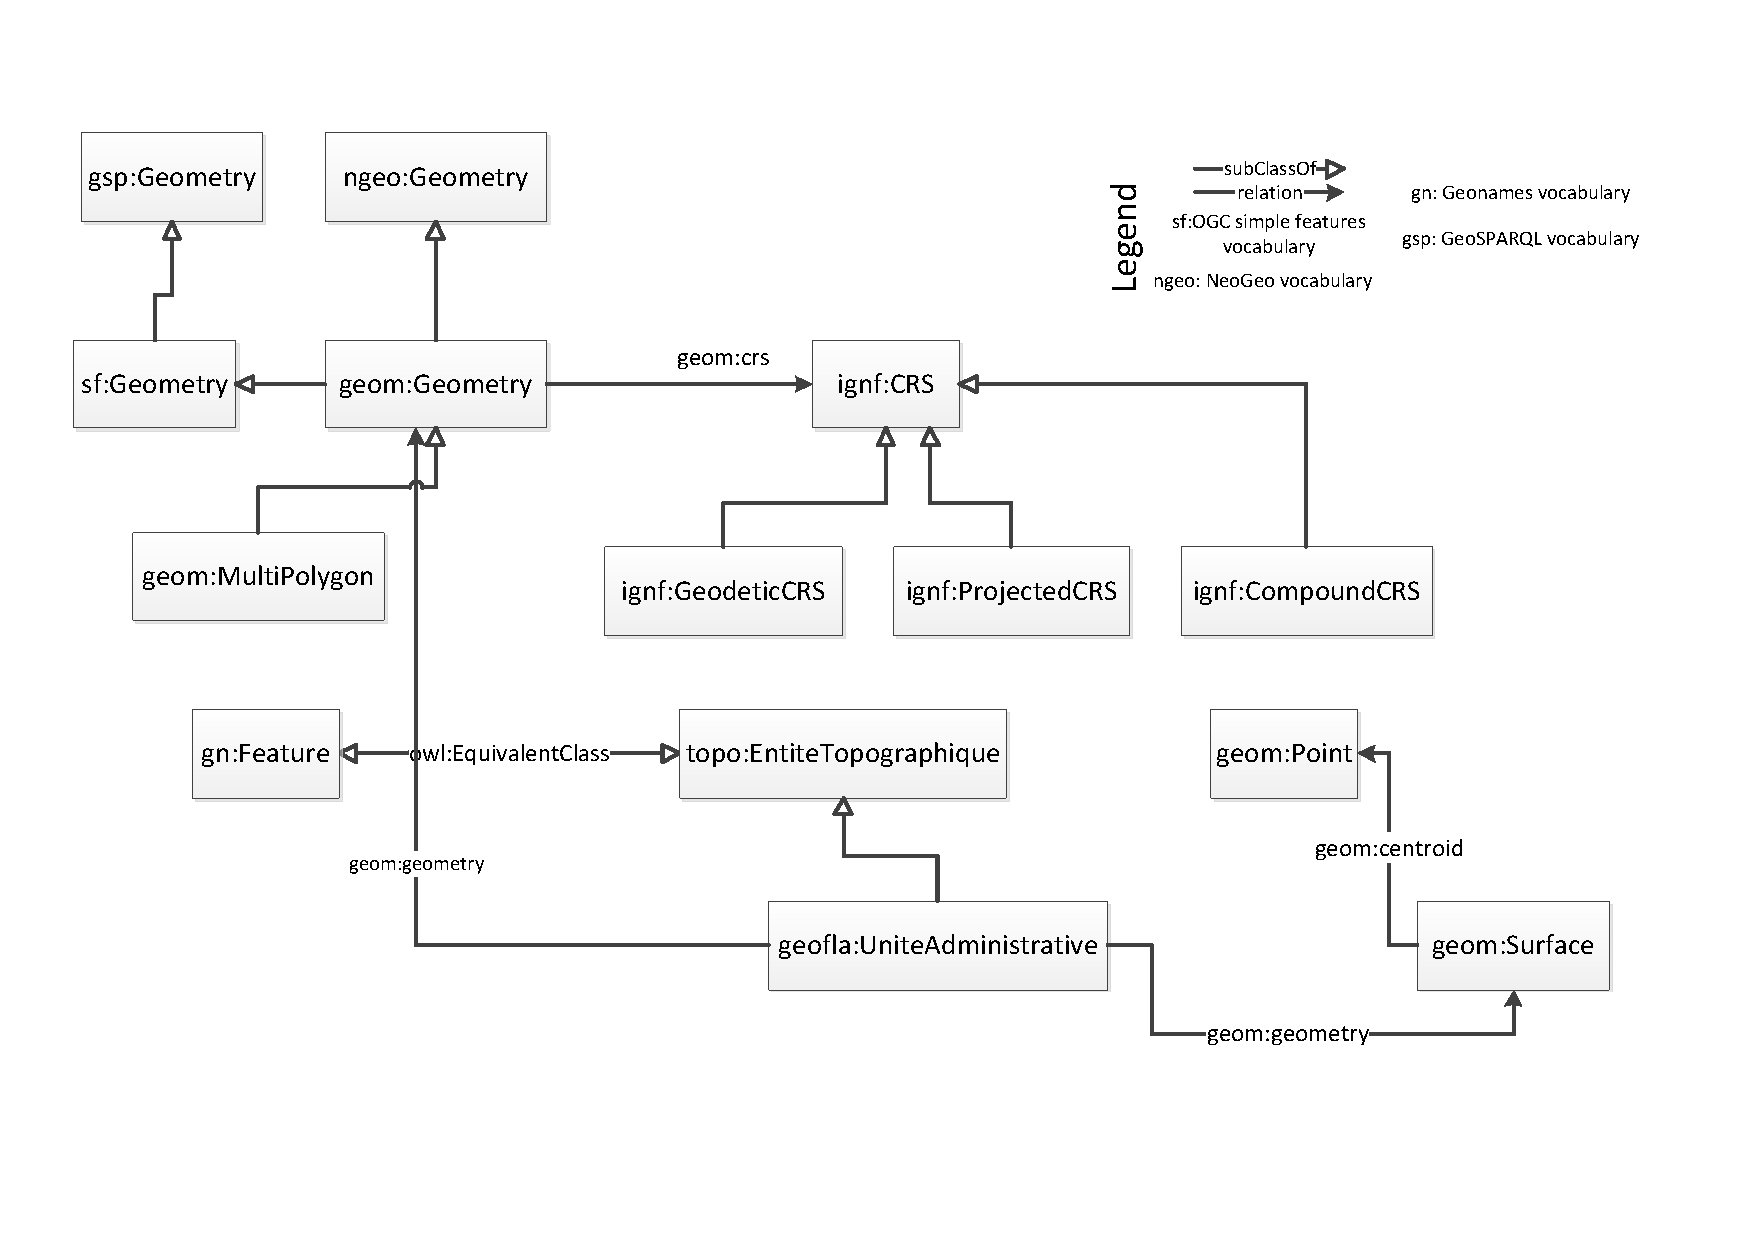
\includegraphics[width=0.8\textwidth]{img/vocabs-ign.pdf}
  \vspace{-15pt}
  \caption{High level classes of ignf, geom and topo vocabularies; relationships between them and mappings with external vocabularies.}
  \vspace{-10pt}
  \label{fig:geomcrs}
  \end{center}
\end{figure}



\subsection{CRS requirements for the  French territory} \label{sec:reqs}

As explained in Section \ref{sec:context}, making explicit the CRS used in a given dataset is a very important issue when dealing with direct location data. This is especially important in the field of geographical information where different CRSs are commonly used due to technical or legal requirements. For INSPIRE Directive, CRS are considered as reference data used for linking thematic data \cite{inspire2009}, and must be described according to ISO 19111 standard. To be consistent with Linked Data principles, CRS should be identified by URIs, like in OGC proposal. Moreover, as Linked Data users are not always familiar with CRS identifiers commonly used within the geographic information community, URI used to identify CRS should use more intuitive names. Finally, consistently with our goal of contributing to a better georeferencing of data on the French territory, we need an access to the descriptions of all French CRSs, including some deprecated but still used CRSs like ``Lambert 1''.


\begin{wraptable}{r}{5.0cm}
\centering{
\scriptsize
\begin{tabular}{lr}
\specialrule{1pt}{1pt}{1pt}
 \textbf{Prefix}	& 	\textbf{URI}	  \\ \specialrule{1pt}{1pt}{1pt}
geofla 	   & \url{http://data.ign.fr/def/geofla#}  \\
geom &  \url{http://data.ign.fr/def/geometrie#} \\
ignf &  \url{http://data.ign.fr/def/ignf#} \\
rgeofla &  \url{http://data.ign.fr/id/geofla/} \\
topo &  \url{http://data.ign.fr/def/topo#} \\
rtopo &  \url{http://data.ign.fr/id/topo/} 

		\\ \specialrule{1pt}{1pt}{1pt}
\end{tabular}
\caption{ URI schemes and conventions used for vocabularies and resources .}
\label{tab:uris}
}
\end{wraptable}

The Information and Service System for European Coordinate Reference Systems\footnote{\url{http://www.crs-geo.eu}}  provides an access to ISO 19111 standard-based descriptions of the main European CRSs but has the same limitation as the EPSG registry: access to the descriptions is not allowed by URI, but only through a cartographic interface.
\url{SpatialReference.org} initiative aims at allowing users to use URI-based references to spatial reference systems, including some CRSs defined and maintained by IGN France.  Besides, the proposed URL policy is not very intuitive. As an example, this URL identifies the projected system defined by IGN France, Lambert 93: \url{http://spatialreference.org/ref/sr-org/7527/}. Moreover, the definitions of some deprecated CRSs such as Lambert zone projected CRSs (which are still used in some datasets) seem to be referenced only for the authority EPSG and not for IGNF, which also maintains a registry of CRSs. ISO 19111 standard-based definitions of all CRSs defined and maintained by IGN France are  published in an XML file\footnote{\url{ http://librairies.ign.fr/geoportail/resources/IGNF.xml}}.
References to equivalent definitions provided by the EPSG registry are explicitly stated with EPSG SRID. CRSs are identified by URIs using short names instead of numeric codes. For example, \url{http://registre.ign.fr/ign/IGNF/crs/NTFLAMB2E}  is the URI designed for the ``Lambert 2 \'{e}tendu'' projected system. Indeed ``NTFLAMB2E'' is used to identify the projected system ``Lambert 2 \'{e}tendu'' which is based on NTF (New French Triangulation) geodetic reference system. Unfortunately, this registry is still in evolution and its URIs are not dereferenceable yet.
 
%\paragraph{Publishing a dataset on French CRSs}
As no existing registry fulfilled all our requirements, we have developed a vocabulary\footnote{\url{http://data.ign.fr/def/ignf}}, inspired from the ISO 19111 schema for CRSs description. Then we have converted IGNF CRSs registry into RDF, and published this dataset on the Web with the Datalift platform\footnote{A service to lookup CRS in RDF can be found at \url{http://www.eurecom.fr/~atemezin/ignf-lookup/}}. Therefore, the description of the ``NTF Lambert 2 \'{e}tendu'' projected CRS can be retrieved at this URL \url{http://data.ign.fr/id/ignf/crs/NTFLAMB2E}.

\subsection{Vocabularies for Geographic Feature Types}
\label{sec:}

Indirect georeferencing of resources on the Web requires reference geographic data on named places and therefore vocabularies for describing feature types and their properties. Therefore, we have chosen to publish a reference dataset on administrative units called GEOFLA\circledR, which is already available in GIS format under an Open Data license. We have also made tests of data conversion and interlinking with another largest dataset on French names places. We have produced and published two vocabularies to describe these datasets, to make sure that all concepts and properties needed would be available.
In the GEOFLA\circledR ~vocabulary\footnote{\url{http://data.ign.fr/def/geofla#}}, 5 classes have been defined: commune, canton, arrondissement, department and region. In the BD TOPO\circledR ~vocabulary\footnote{\url{http://data.ign.fr/def/topo}} $35$ main classes have been defined. They represent the main types of geographic features represented in the BD TOPO\circledR ~database. In both vocabularies, properties have been defined based on the attributes of their related classes in the databases. The geographic feature types defined as values of attributes ``nature'' are modeled as instances of \texttt{skos:Concept}. SKOS is intensively used to easily group concepts into different schemes (using \texttt{skos:hasTopConcept}) and provide semantic relationships (e.g: \texttt{skos:broader}, \texttt{skos:narrowMatch}) among them. We also provide alignments with Geonames vocabulary, where \texttt{topo:Place} is subclass of \texttt{gn:S} and \texttt{owl:sameAs} linked concepts.\footnote{\url{https://github.com/gatemezing/ign-iswc2014/blob/master/vocabularies/mappingsGeonames.ttl}} 

All the classes are defined as subclasses of  \texttt{topo:EntiteTopographique} which defines the representation of a real world entity associated to a location relative to the Earth, consistently with ISO TC 211 and OGC standards. 
The GEOFLA\circledR 's application schema is composed of classes representing different types of french administrative units, namely communes, cantons, arrondissements and departments. In \texttt{geofla} vocabulary, we add a class region  from the instances of the class department via two attributes  that precise to what region each instance of department belongs.  Their properties are defined based on the attributes of their related classes in GEOFLA\circledR ~database.

Regarding use cases consuming  real-world databases developed using the vocabularies aforementioned, two different applications have been developed. namely \textit{PerfectSchool}\footnote{\url{semantics.eurecom.fr/datalift/PerfectSchool/}}  and \textit{Equipment}\footnote{\url{http://semantics.eurecom.fr/datalift/Equipment/}}. The former is a mobile application intended to provide useful information on schools in France, while the latter is a facet view by categories of facilities in France, specifically in the city of Toulouse. 
A Commune has an attribute called \textit{``nature''} whose enumerated values precise whether the commune is the capital of a bigger administrative unit, modeled in the vocabulary by the ObjectProperty \texttt{geofla:statut} with range \texttt{skos:Concept} defined in this specific \texttt{skos:ConceptScheme} \url{http://{BASE}/codes/geofla/typedecommune/liste} pointing to the different types of French administrative unit's capital. 

\textcolor{red}{
\subsection{Publishing structured geometries from geographic data}
The vocabulary for geometry reused by a geodata converter that takes traditional GIS data as input and outputs RDF data with geometries defined both with a \texttt{gsp:wktLiteral} and with a structured representation compliant with our vocabulary. Geometries are automatically associated with the chosen CRS. This converter is implemented as a plugin of the Datalift platform and can be reused easily for geographic data publishing purpose.
}

\clearpage


\chapter{Crowd level estimation using texture features}
\label{ch:ch2}

\clearpage

\chapter*{Part 2 - Generating Visualizations for Linked Data}
\label{part:part2}
 \vspace{10mm}
\section*{Summary}
This part cover three main problematics regarding how to present RDF to end-users. There is a consensus that RDF is not what is shown to the users.  First, we make a state of the art review of existing tools and solutions for visual representation and exploration of RDF (Visualbox, LODSpeaKr, Map4RDF, Linked Data Visualization Model, other works from the SWUI community, from Roberto Garcia, etc.) The, we present our contribution: the wizard for visualizations including the vocabulary for describing visualizations , the prototype itself, etc. Third, we present a  mechanism of extracting and reusing application contests in open data events, and finally we provide some insights on revealing the important properties of Entities for visualization. 

\chapter*{Part 3 - Contribution to Standards}
\label{part:part3}
 
 \vspace{10mm}
\section*{Summary}
In this part, we present the various work and contributions around the Linked Open Vocabularies ( catalog description, vocabulary publications, APIs and endpoints); prefixes harmonization, vocabulary ranking metrics using information content. We also present some insights on checking licenses compatibility between vocabularies and datasets with the defeasible deontic logic for creating an automatic tool for licenses checking.  We then finish by highlighting our contribution to the GLD WG with the 2 document notes and vocabularies standardized: DCAT, Data Cube, ORG, etc. 
 
%\clearpage




\chapter{Conclusions and Future Perspectives}
\label{ch:conc}



\appendix
\include{Appendix1}
%\include{Appendix2}
%\include{Appendix3}

%

\bibliographystyle{plain}
\bibliography{thesis}
\nocite{*}
\printnomenclature

\chapter*{}
\chaptermark{}
%\section*{}
%\sectionmark{}
\vspace{-15ex}
\appendix
\end{document}
 
